\chapter{Introduction}
In recent years, advancements in technology have significantly increased the capacity for data collection across all sectors. However, these improvements have also resurrected longstanding issues associated with managing large volumes of data, such as inefficiencies in transportation networks and data processing centers.

The adoption of edge/fog computing paradigms has addressed these challenges by decentralizing data processing. Edge computing involves processing data directly at the source, while fog computing processes data at intermediate nodes within the network. This approach enhances the speed and accuracy of data monitoring and consumption systems by reducing the burden on transportation and central processing nodes.

Moreover, these paradigms facilitate the implementation of new functionalities, such as enabling infrastructure to operate independently (island-mode) when disconnected from the main network. They also increase flexibility by allowing data flows to be rerouted to alternative destinations in response to failures. 

Since data is partially processed at distributed nodes, there is less reliance on highly specialized or memory-intensive destination centers, thereby supporting the creation of multiple destination points.

\section{Energy section}

In Italy, the national electrical grid can be divided into four main areas, as highlighted in Figure \ref{fig:macroaree}.

\begin{figure}[ht]\centering
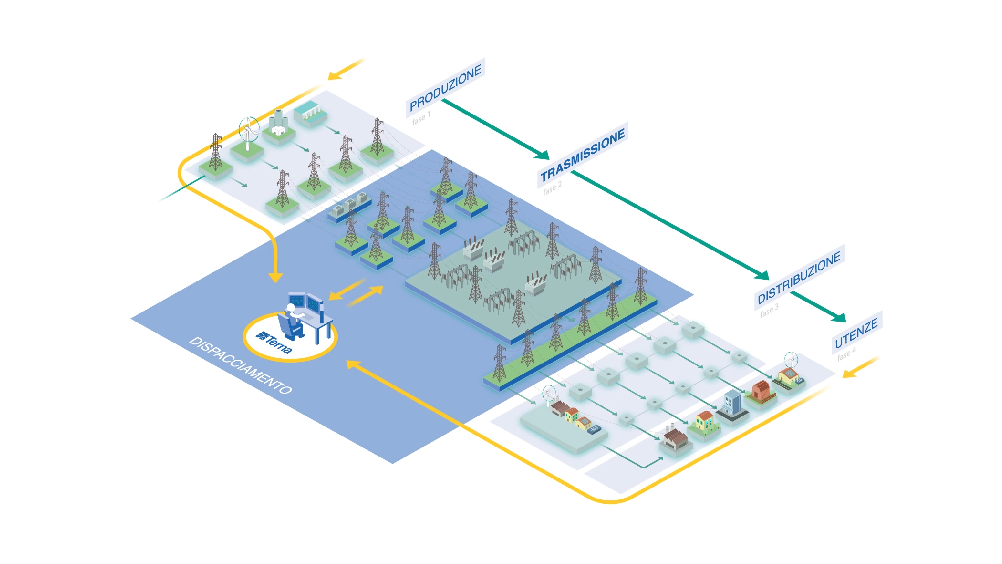
\includegraphics[scale=0.8]{Pictures/macro-aree}
\caption[General Overview of the Electric Energy Grid Macro Areas]{General Overview of the Electric Energy Grid Macro Areas\footnotemark. }\label{fig:macroaree}
\end{figure}


\begin{itemize}
\item \textbf{Production:} This area encompasses all energy production facilities, historically dominated by large power plants such as fossil fuel and hydroelectric plants, as well as imported energy. Nowadays, smaller-scale and more variable production outputs from renewable energy sources have been introduced.
\item \textbf{Transmission:} This area includes the infrastructure responsible for long-distance transmission of produced energy, using high-voltage alternating current. Its primary function, known as "dispatching"\cite{i1-1}, is to balance consumption levels with supply levels since energy cannot be efficiently stored. Managed in Italy by Terna\cite{i1-2}, this infrastructure is highly automated to handle power plant failures or service interruptions.
\item \textbf{Distribution:} This area comprises the infrastructure that transports electrical energy to end-users, passing through primary substations (transforming high-voltage electricity to medium voltage) and secondary substations (from medium voltage to low voltage). It is divided into zones managed by independent distribution companies responsible for maintenance. The Smart Grid model, developed over the past decade, aims to automate this infrastructure similarly to the transmission area to enhance energy control and usage.
\item \textbf{Consumers:} This area involves delivering electricity to the final customer, determining economic costs, and the characteristics of the supplied energy. These aspects are managed by various sales companies that negotiate agreements with distributors and end-users.
\end{itemize}

\footnotetext{\url{https://www.terna.it/it/sistema-elettrico/ruolo-terna/come-funziona-sistema-elettrico}}

Each area plays a crucial role in the overall operation and management of Italy's electricity network, ensuring efficient and reliable energy supply across the country.

\section{Thesis objectives}
The Smart Grid model converts the entire traditional distribution network into an intelligent information network. It integrates edge/fog computing principles and introduces new functionalities such as supporting island-mode operation and securely managing various energy sources through centralized automation.

Current approaches propose using the Kubernetes platform with multi-master clusters to manage individual stations. While these solutions introduce edge/fog computing and local centralized control, they face challenges in scalability, security, and cannot support critical features like island-mode operation across the entire network.

Building on the feasibility of local Kubernetes solutions in distributed environments, this thesis aims to develop a model that extends edge/fog computing capabilities across the entire power grid. 

The innovative open-source project Liqo will be utilized to manage the distributed cluster architecture, enhancing resilience by enabling the system to withstand failures of entire clusters.

\section{Overview}
This thesis endeavors to create a scalable model for the entire network, building upon successful local solutions.

\noindent Chapter 2 introduces Kubernetes, an open-source platform, with a focus on its lightweight version, k3s, as the foundational technology. 

\noindent Chapter 3 delves into the local solution based on Kubernetes, detailing its components and addressing scalability and functionality challenges.

\noindent Chapter 4 introduces the Liqo project, pivotal for extending the local model across the entire network, elucidating its core concepts. It examines how this technology interacts with existing distributed database systems designed for single-cluster environments, emphasizing the adjustments needed for seamless integration.

\noindent From Chapter 5 onward, the thesis delves deeper into its core discussions. Chapter 5 initiates by outlining the rationale behind selecting the partial mesh star physical topology, exploring various hierarchical configurations within this framework and analizing those configuration in term of scalability and resilience. 

\noindent Chapter 6 then presents two viable implementations of this model, tailored to the structure of energy distribution grids.

\noindent Chapter 7 critically evaluates the first implementation chosen for its robust resilience, contrasting its performance against the initial local solution. 

\noindent Finally, Chapter 8 provides a reflective analysis of the findings and proposes future research directions.








